\subsection{制御系}
制御系は、植松電機どの所有の設備を用いた。ニクロム線加熱スイッチ、開放弁スイッチ、パージベンスイッチ、冷却弁スイッチにより構成されている。ニクロム線加熱時間、加圧弁開放時間、開放弁開はタイマーにより制御可能である。
\\
供試体1を使用した燃焼気化実験では、ニクロム線を加熱を開始した後に、LOXタンクの自己加圧によりインジェクタから放出される酸素と燃料が着火したことをビデオモニタにより確認した時に、加圧弁スイッチをオンにし、本着火を開始した。
規定の加圧弁開時間を終了したところで、加圧弁が閉じられて、開放弁が開となりLOXタンク圧力が開放される。それと同時に手動でパージ弁を開とし、窒素によるパージを行う。
供試体2を使用した燃焼気化実験では、外殻をステンレスで覆っているため、ノズル上流温度が上昇し始めたら着火したと判定し、加圧弁スイッチをオンにした。その他の手順は供試体1での実験と同様である。
ニクロム線設置位置を図\ref{fig:Nichrome}、着火判定した点を図\ref{fig:Ignition}
\begin{figure}
\centering
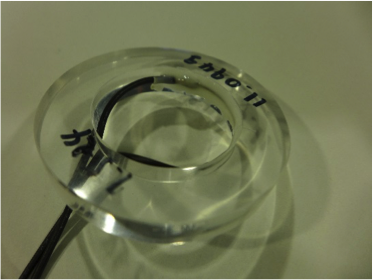
\includegraphics[width=10cm]{\FigAddTwo/Nichrome.png}
\caption{ニクロム線}
\label{fig:Nichrome}
\end{figure}
\begin{figure}
\centering
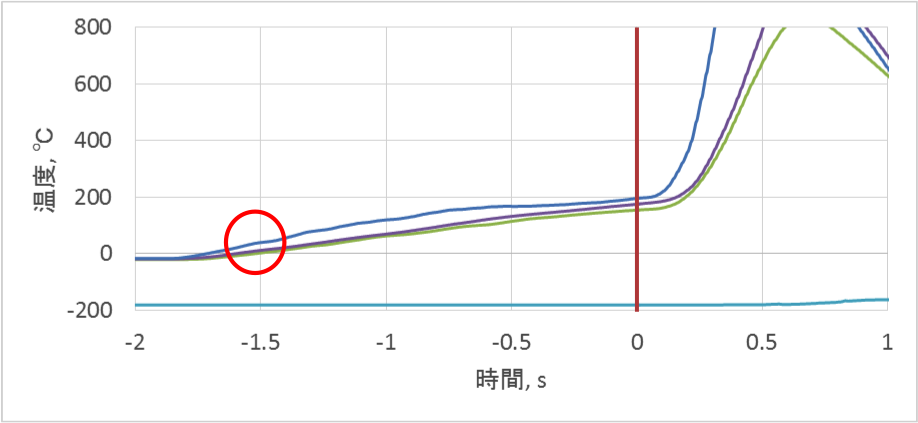
\includegraphics[width=11cm]{\FigAddTwo/Ignition.png}
\caption{着火判定した点}
\label{fig:Ignition}
\end{figure}
